\documentclass{standalone}
\usepackage{tikz}
\usepackage{ctex,siunitx}
\setCJKmainfont{Noto Serif CJK SC}
\usepackage{tkz-euclide}
\usepackage{amsmath}
\usetikzlibrary{patterns, calc}
\usetikzlibrary {decorations.pathmorphing, decorations.pathreplacing, decorations.shapes,}
\begin{document}
\small
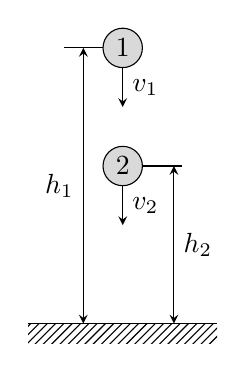
\begin{tikzpicture}[>=stealth,scale=1]
  \fill [pattern = north east lines] (-.2,-.25) rectangle (2.2,0);
  \draw (-.2,0)--(2.2,0);
  \draw [fill=gray!30] (1,3.5) node {1} circle (.25) ;
  \draw [fill=gray!30] (1,2) node {2} circle (.25) ;
  \draw (.75,3.5)--(.25,3.5);
  \draw (1.25,2)--(1.75,2);
  \draw [<->] (.5,3.5)--node[left] {$h_1$} (.5,0);
  \draw [<->]  (1.65,2)--node[right] {$h_2$} (1.65,0);
  \draw [->](1,3.25)--node[right] {$v_1$} (1,2.75);
  \draw [->](1,1.75)--node[right] {$v_2$} (1,1.25);
\end{tikzpicture}
\end{document}